\newpage

\section*{ Gold  (Cd) }

Power Level: 100 kW(th) \\
Time at Power: 45 s \\
Wait Time: 300 s \\
Total Activity at Removal: 2.49e+03 $\mu Ci$

\begin{table*}[h]
\centering
\begin{tabular}{ |c|c|c|c|c|c|c| }
 \hline
 Position & Mass $mg$ & Start Counting $s$ & Counting Time $s$ & Counting Activity $\mu Ci$ \\
 \hline 
 1 & 5.0 & 345 & 300 & 2.28e+01\\ 
\hline
 2 & 4.35 & 645 & 300 & 1.98e+01\\ 
\hline
 3 & 4.3 & 945 & 300 & 1.96e+01\\ 
\hline
 4 & 4.37 & 1245 & 300 & 1.99e+01\\ 
\hline
\end{tabular}
\end{table*}

\begin{figure}[!ht]
   \centering
   \subfloat[][Position \#1]{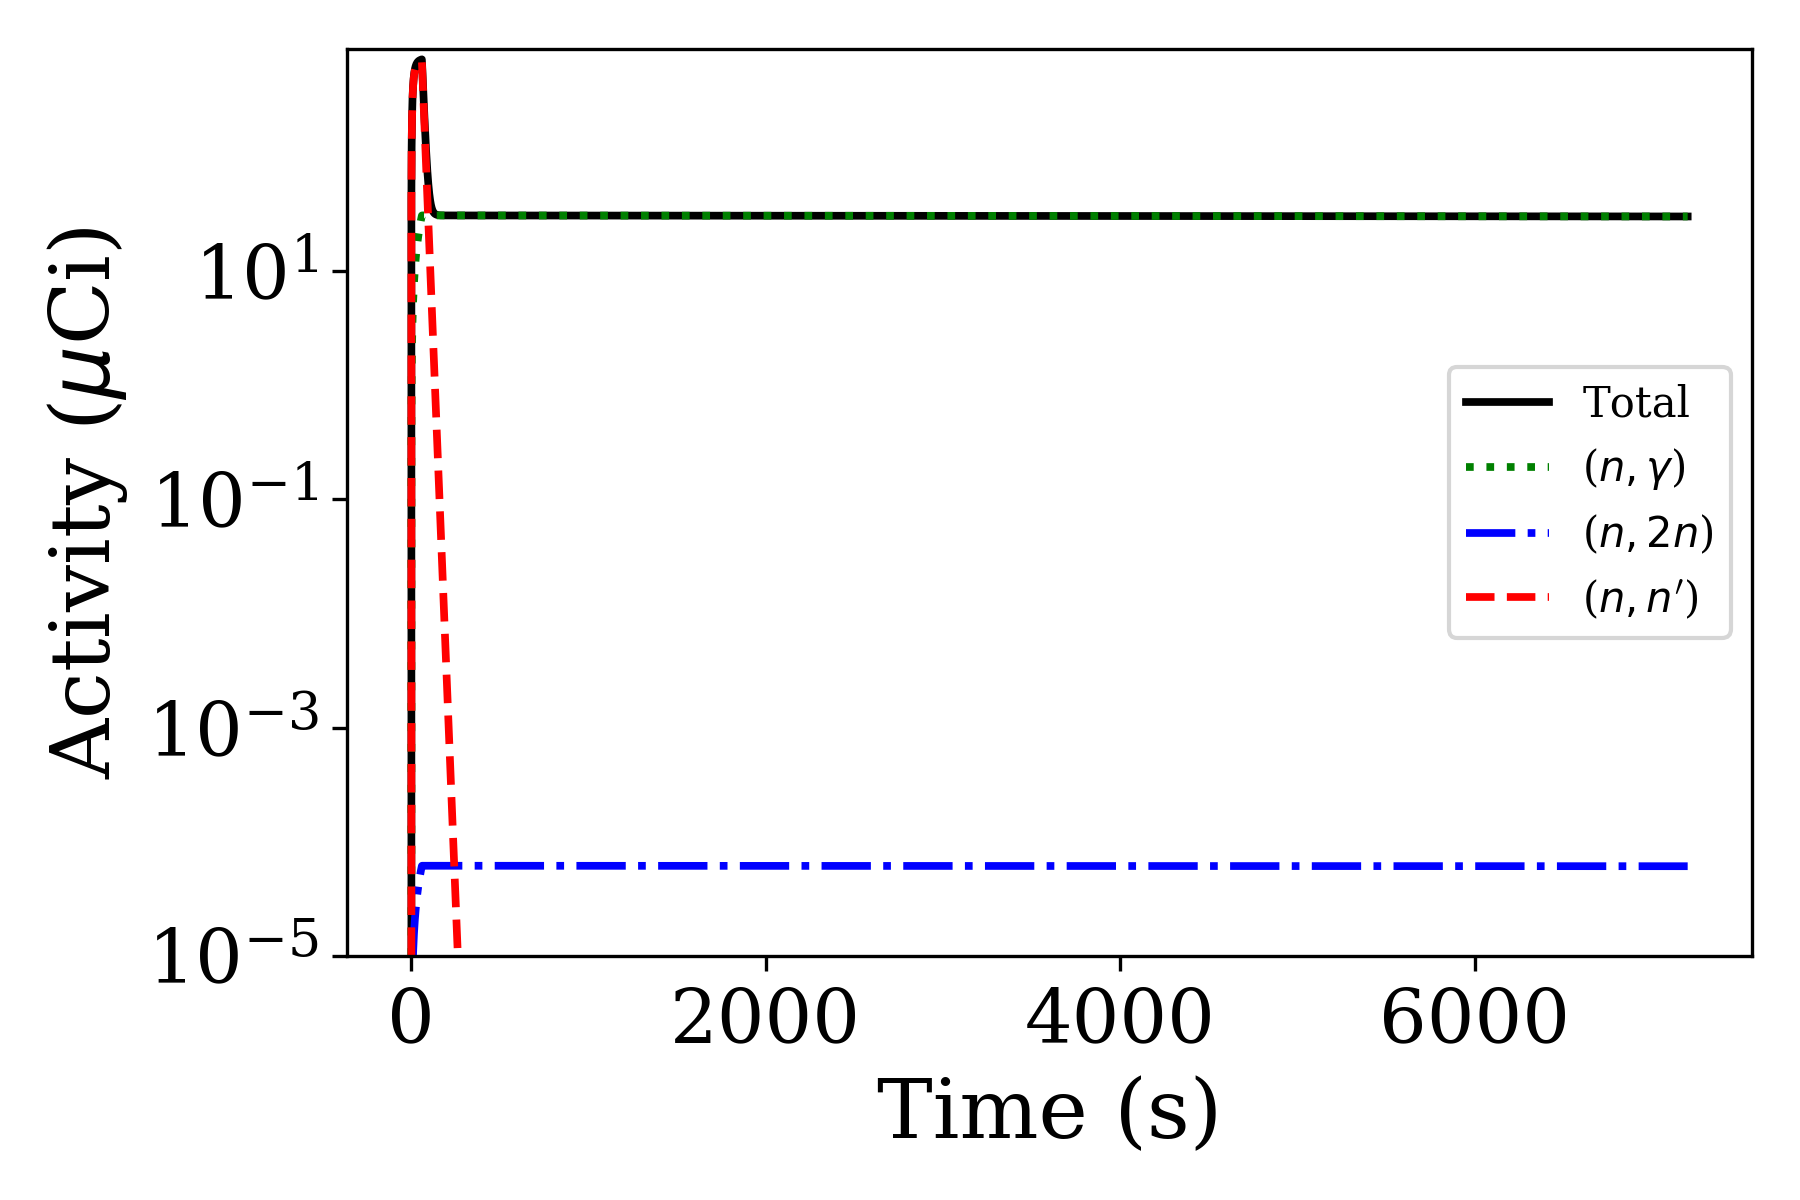
\includegraphics[width=.4\textwidth]{source/plot/au1cd_activity}}\quad
   \subfloat[][ ($n,\gamma$) Reaction Rate]{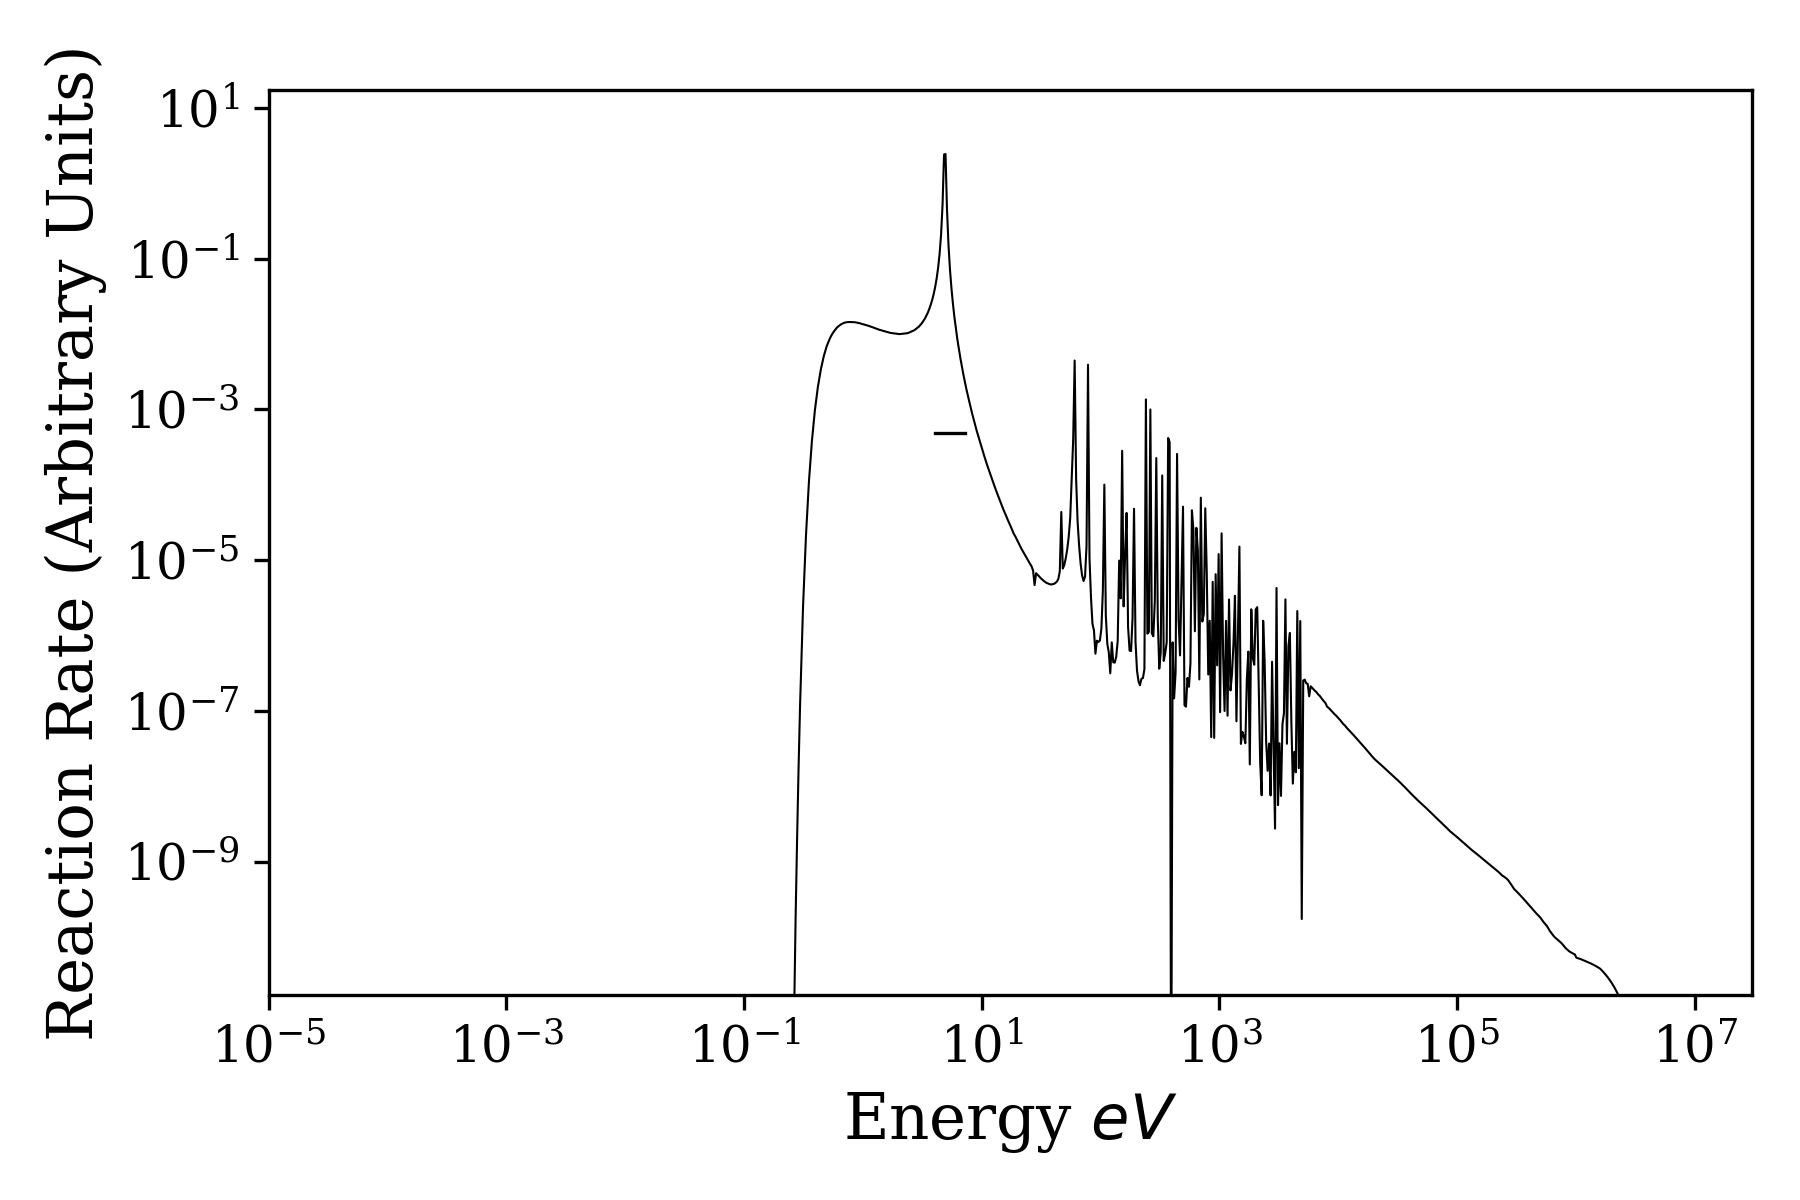
\includegraphics[width=.4\textwidth]{source/plot/au_n,gamma_cd}}\\ 
   \subfloat[][ ($n,2n$) Reaction Rate]{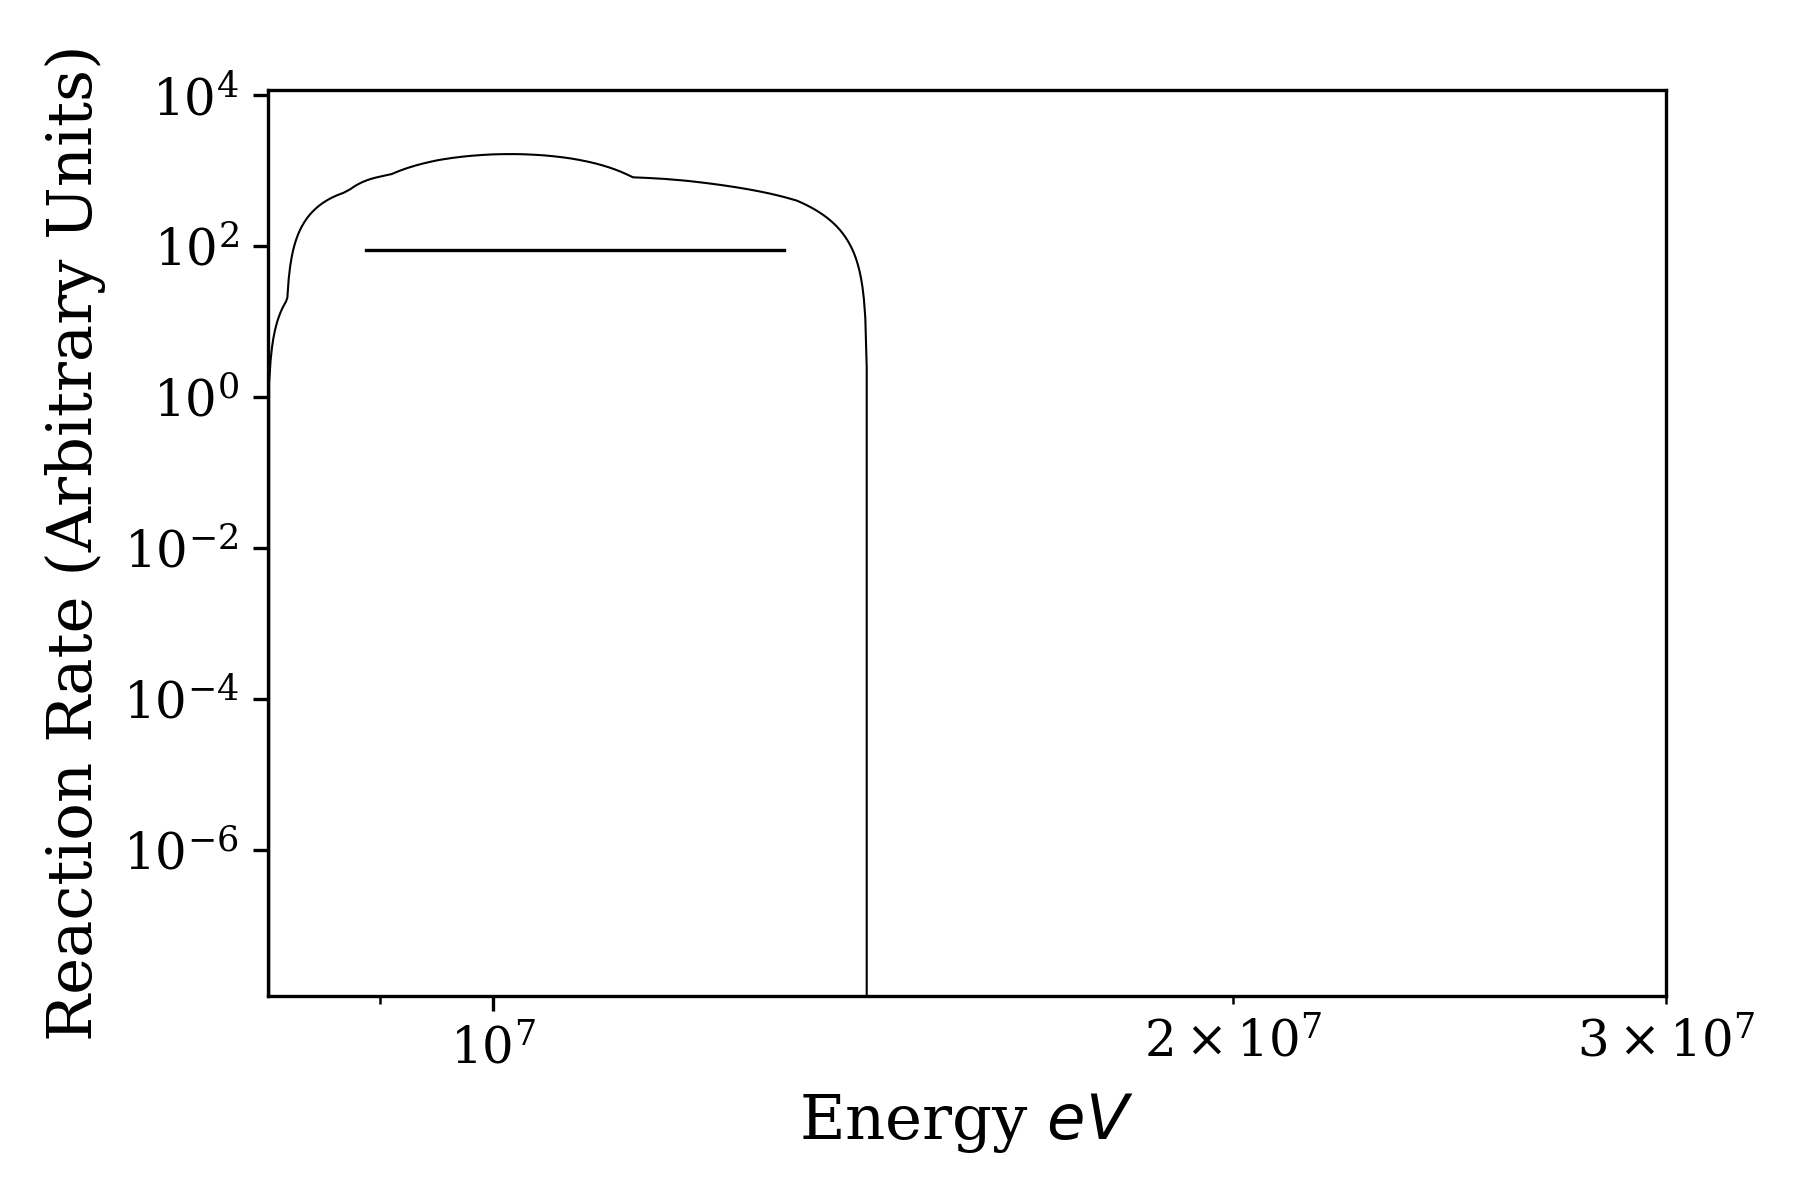
\includegraphics[width=.4\textwidth]{source/plot/au_n,2n_cd}}\quad 
   \subfloat[][ ($n,n'$) Reaction Rate]{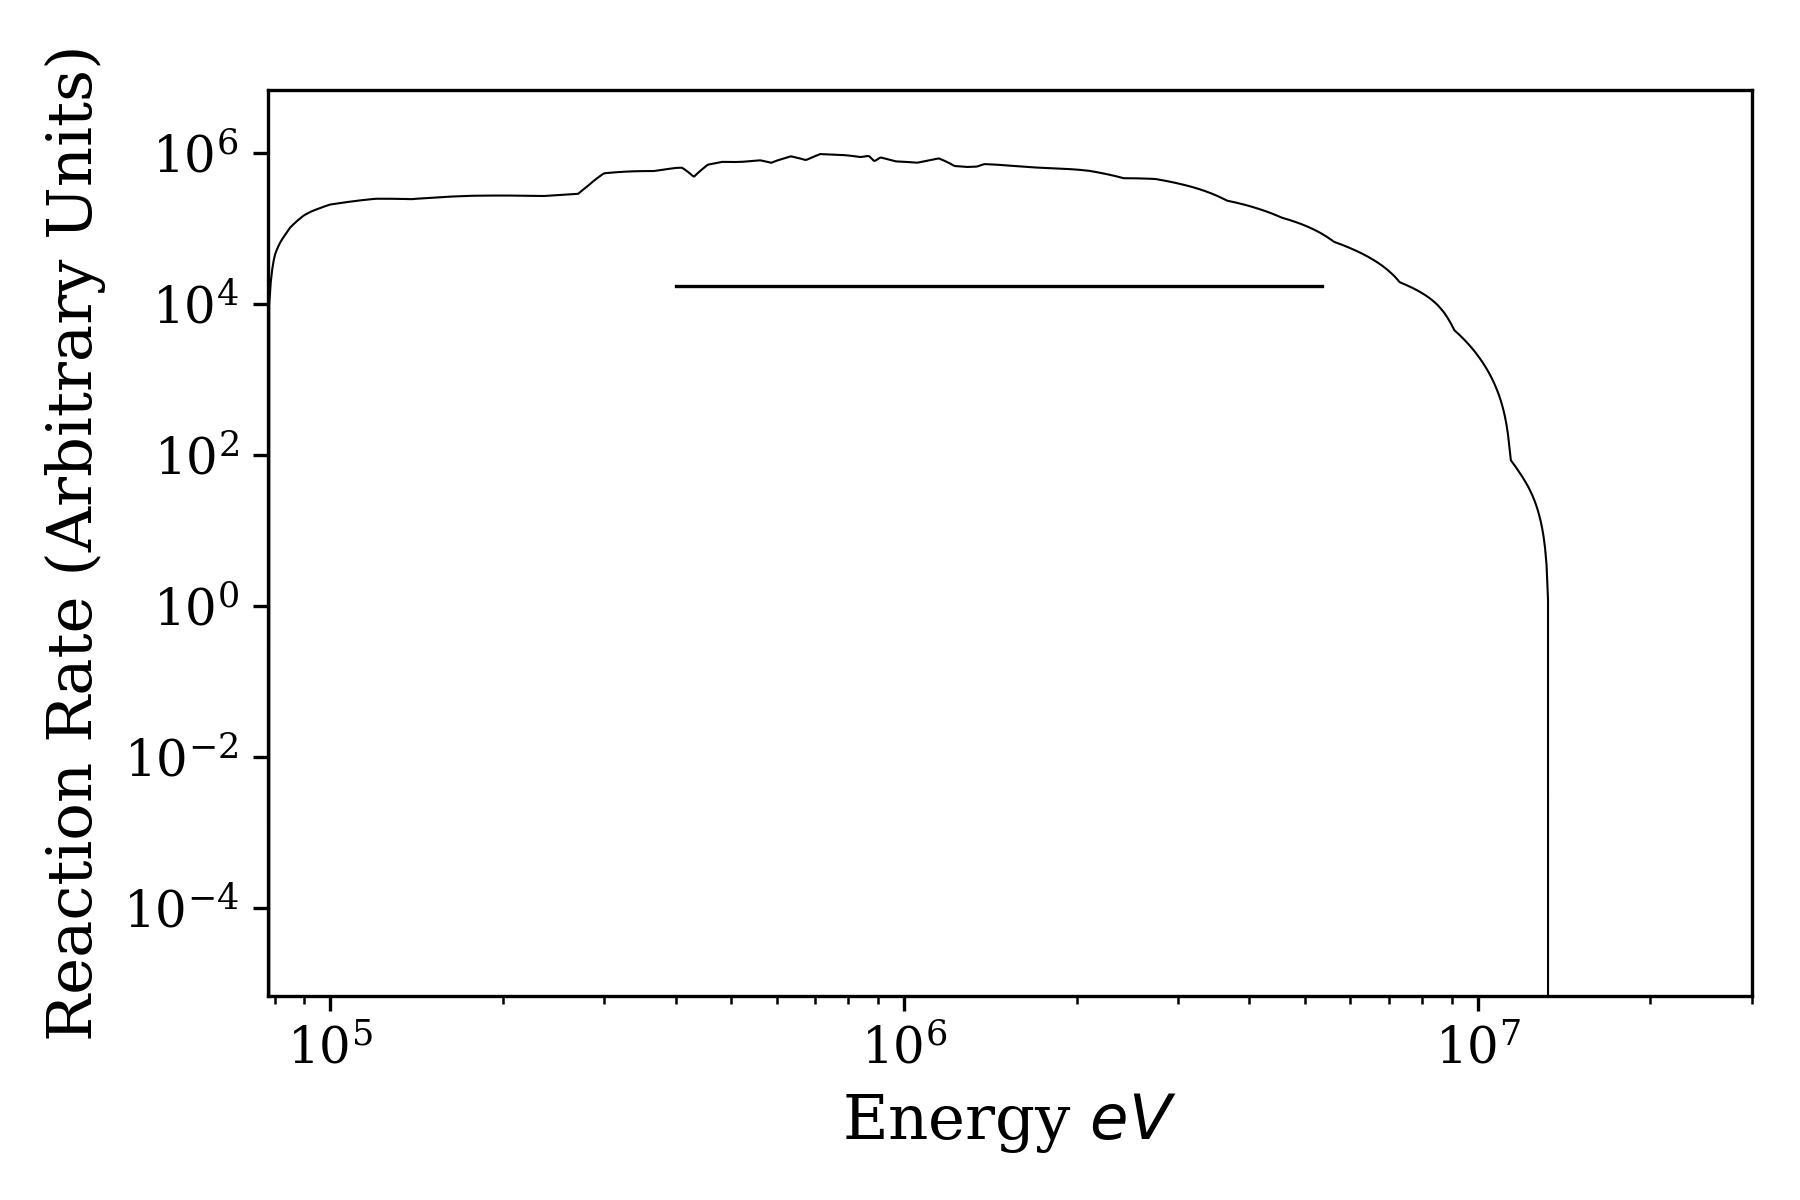
\includegraphics[width=.4\textwidth]{source/plot/au_n,inelastic_cd}}\\ 

\end{figure}

\begin{table*}[h]
\centering
\begin{tabular}{ |c|c|c|c|c|c|c| }
 \hline
 Reaction & T$_{1/2}$ & ROI (eV) & Important Gammas (keV) \\
 \hline 
 ($n,\gamma$) &  2.7 d & 4.08e+00, 7.17e+00 & 412(0.95), 676(0.01), 1088(0.002) \\ 
\hline
 ($n,2n$) &  6.2 d & 8.83e+06, 1.35e+07 & 333(0.25), 356(0.94), 426(0.06), 1091(0.002) \\ 
\hline
 ($n,n'$) &  7.8 s & 3.28e+05, 5.28e+06 & 130(0.08), 279(0.75) \\ 
\hline
\end{tabular}
\end{table*}
